\subsection{Repräsentativer Anwendungsfall für die Energiewirtschaft}\label{usecase}

Die verschiedenen Werttreiber und Anforderungen für ein Digitalisierungskonzept unterscheiden sich je nach Unternehmen und Branche.
Für eine erfolgreiche Transformation müssen daher individuelle Anwendungsfälle identifziert werden.
In Anbetracht der Dynamik und des rasanten Tempos, in der neue Technologien entstehen,
ermöglicht ein anwendungsfallbasierter Ansatz eine flexible und agile Anpassung. \citep[S. 31]{Acharya2019}
\\Aus diesen Gründen wird im Folgenden ein repräsentativer Anwendungsfall für die Energiebranche vorgestellt. Die Anforderungen an das Zielsystem werden nach den von \citet{Lauenroth2016} vorgestellten Methoden erhoben.

\subsubsection{Ausgangsszenario} \label{usecase}

Der Windenergieanlagenhersteller Enercon GmbH aus Aurich verzeichnet 29000 Anlagen in 45 Ländern. Da das Kerngeschäft des Unternehmens auf den Bau von Anlagen für die dezentrale Energieerzeugung basiert, hat Industrie-4.0-Fähigkeit einen besonderen Stellenwert. Sei es die Einspeisung der produzierten Energie in das Smart-Grid, die Fernsteuerung oder die Zustandsüberwachung der Anlagen und Windparks: Das unternehmenseigene \acf{scada}-System ist auf die Enercon-Anlagen abgestimmt bietet umfangreiche Lösungen für die Kunden. Allerdings versendet das \ac{scada}-System die Messwerte bisher nur alle 15 Minuten das \ac{cms}. Zudem ist es eine technische Insellösung, welche die betriebwirtschaftliche Welt nicht integriert. Als Kunden stehen die Energieversorgungsunternehmen im Vordergrund, mit denen Enercon Verträge für Wartungsservices abschließt. Die Enercon-IT nutzt SAP-Produkte für das Management der Ressourcen,Logistik oder Kunden. Im Zuge der Anpassung an die Anforderungen der digitalen Welt wird SAP jedoch den Support der bisher auch von Enercon verwendeten Standard-ERP-Software bis 2025 einstellen. Der Fokus wird auf das Nachfolgeprodukt SAP S/4 HANA gesetzt, welche die echtzeitfähige In-Memory-Datenbanktechnologie \acf{hana} für nutzt. Aus diesem Grund bereitet sich Enercon rechtzeitig auf die Migration auf S/4 HANA vor. Die Integrations- und Entwicklungsplattform von \ac{hana} bietet zahlreiche Möglichkeiten zur Realisierung von innovativen Softwarelösungen sowohl auf der Cloud als auch On-Premise. Die Neuausrichtung der IT-Architektur ist auch für die erfolgreiche digitale Transformation von Enercon großer Bedeutung.

\noindent Im besonderen Interesse liegt die SAP Leonardo \ac{iot} Foundation, vor allem in Anbetracht einer möglichen Integration von Stammdaten aus dem S/4 HANA System. Dafür ist zunächst eine Analyse der SAP Leonardo Systemarchitektur mitsamt der Perspektiven gewünscht. Dies könne als Entscheidungsgrundlage für eine Erweiterung des Geschäftsfeldes von Energieproduktion auf IT-Dienstleistungen dienen. Außerdem soll prototypisch dargestellt werden, inwiefern sich SAP Leonardo IoT als Verwaltungsschale für die Industrie-4.0-Komponente eignet. Langfristiges Ziel des Unternehmens sei es, das \ac{scada}-System echtzeitfähig zu gestalten. Um Risiken vor Inbetriebnahme und Kosten zu minimieren soll jedoch zunächst eine einfache Simulation genügen.

\noindent Die Simulation soll dem Servicepersonal in der Wartung und den Kunden ermöglichen, die Zustandsdaten des digitalen Zwillings einer Anlage in Echtzeit zu überwachen. Wenn kritische Messwerte empfangen werden, soll das Personal sofort benachrichtigt werden, damit Wartungsmaßnahmen eingeleitet werden können. Die Softwareentwickler/innen sollen den Prototypen beliebig sowohl um (Mess-)Geräte als auch um App-Funktionalitäten erweitern können.

\subsubsection{Anforderungserhebung}

Um die Anforderungen für die Umsetzung einer repräsentativen Lösung zu bestimmen, muss zunächst ermittelt werden, welche Einflussfaktoren sich im Kontext des Zielsystems befinden und wo sich die Grenze des Systems befindet. Mit der Evaluation der Ausgangssituation (s. \ref{usecase}) können Anforderungsquellen identifiziert werden, welche sich auf das Zielsystem beziehen und sich im Systemkontext befinden (s. Abbildung \ref{kontext}). Auf Grundlage der Evaluation werden zunächst Probleme, Anforderungen und Lösungen für das System definiert. Für eine bessere Strukturierung des Systems werden die einzelnen \ac{pal} auf die Ebenen System und Systemkontext, sowie auch auf die technische Ebene abstrahiert. Die Dokumentation von Anforderungen auf verschiedenen Abstraktionsebenen ist vor allem für die nachträgliche Verwaltung der Anforderungen für zukünftige Softwareprojekte von großem Wert \citep{Lauenroth2016}. Nach \citet{IREB2017} unterscheidet man typischerweise zwischen drei Arten von Anforderungen: funktionale Anforderungen, Qualitätsanforderungen sowie Randbedingungen. Die funktionalen Anforderungen werden weiter in verschiedene Perspektiven unterteilt. Aus der Struktur- bzw. Datenverspektive wird die Struktur der Ein- und Ausgabedaten beschrieben, welche in der Funktionsperpektive verarbeitet werden. Die Verhaltensperspektive beschreibt das Verhalten des Systems auf Basis von Zuständen und Ereignissen \citep{Lauenroth2016}.
Daraufhin werden aus den ermittelten Anforderungen Teilsysteme identifiziert, für welche die Anfoderungen ebenfalls nach dem \ac{pal}-Model erfasst werden. Die Formulierung von Anforderungen setzt das Vorhandensein einer Lösung voraus, weshalb auch der Prototyp bereits als Anforderungsquelle gelten kann.
\\\\Aus der Evaluation der Ausgangssituation ergibt sich die in Abbildung \ref{kontext} dargestellte Systemabgrenzung. Die Anforderungsanalyse berücktsichtigt die Stakeholder, welche sowohl mit dem System interagieren als auch direkten Einfluss auf die Anforderungen haben. Als Nutzer des Systems kristallisieren sich die Kunden Enercons (z.B. die \ac{evu}) sowie das Servicepersonal, welches in der Wartung tätig ist. Stakeholder, welche eher qualitative Anforderungen an das System stellen, sind die Softwareentwickler/innen und -architekt(inn)en, für welche der Prototyp als Architekturvorlage dienen soll. Die Auftraggeber stellen die direkte Anforderung, eine Lösung und Analyse für SAP Leonardo zu entwickeln, die die Eignung SAP Leonardos als Verwaltungsschale für die Industrie-4.0-Komponente beurteilt. Dies impliziert, dass sich an der IT-Sicht (s. Abbildung \ref{it_layer}) der Referenzarchitektur RAMI 4.0 und an dem Konzept der Industrie-4.0-Komponente (s. Abschnitt \ref{rami}) orientiert werden soll. Berücksichtigt werden sollen außerdem die Anforderungen, die sich aus der Beschaffenheit der Branche der Energiewirtschaft ergeben. Bereits existierende Systeme können ebenfalls Einfluss auf das System haben, was jedoch für die Prototypentwicklung nicht relevant ist.


\begin{figure}[h]
  \centering
  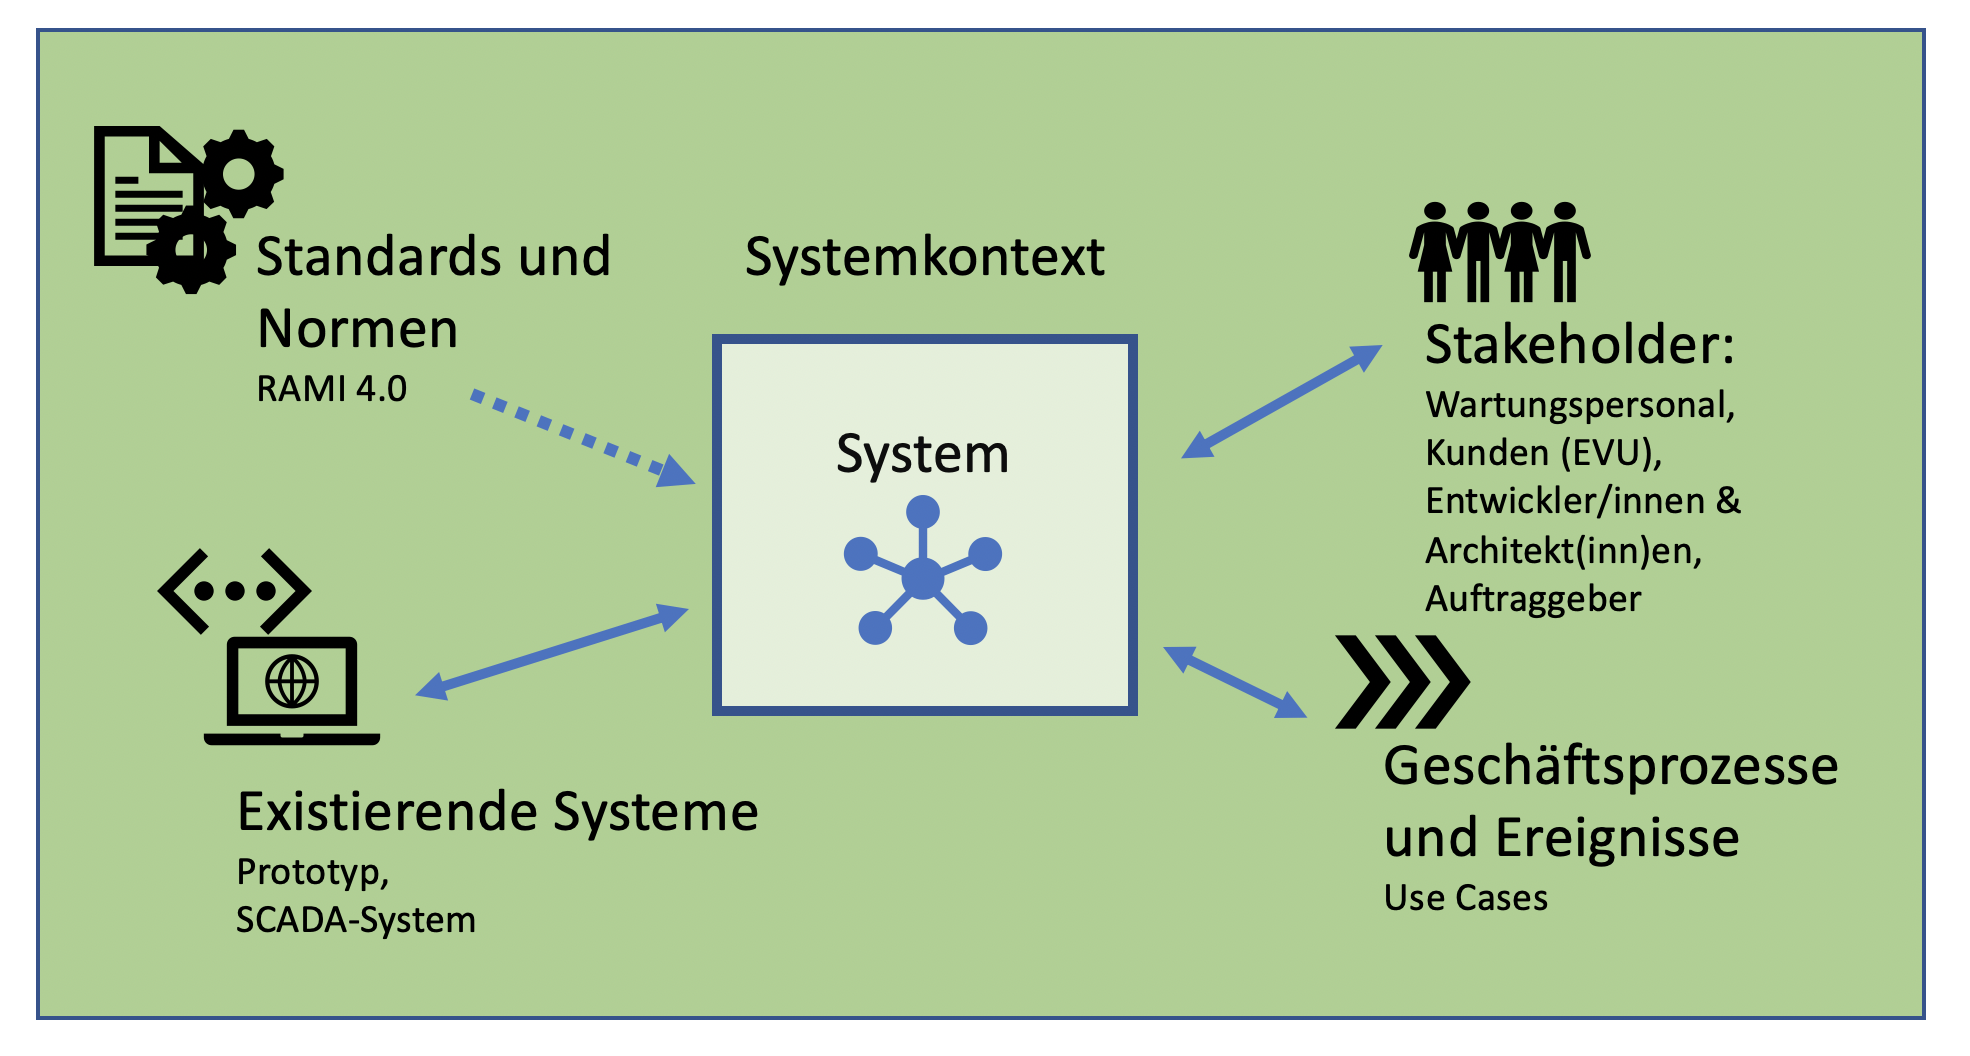
\includegraphics[width=1\linewidth]{System_Kontext.png}
  \caption[Systemabgrenzung und Systemkontext]{Systemabgrenzung und Systemkontext}
  \label{kontext}
\end{figure}

% Anforderungsanalyse ***********

\subsection{Anforderungsanalyse}
Im folgenden Kapitel wird die Anforderungsanalyse nach Abstraktionsebenen des \ac{pal}-Modells (s. Tabelle \ref{pal}) durchgeführt. In der Kontextebene werden Anforderungen bestimmt, welche sich direkt oder indirekt die Funktionen des Systems bestimmen. Es werden Einflussfaktoren behandelt, welche sich außerhalb der Systemgrenzen befinden. Die Behandlung der Forschungsfrage FF1.1, welche Anforderungen an ein System für die digitale Transformation sich aus Sicht der dezentralen Energierzeugung ergeben, schafft die Grundlage für die Problemdefinition für die Funktionsweise des eigentlichen Systems. Die Funktionen werden in der Systemebene mit den notwendigen Schnittstellen und Datenstrukturen in einen logischen Aufbau eingeordnet. Anschließend wird auf der technischen Ebene der logische Aufbau technisch beschrieben.

\newpage

\begin{table}[h]
  \begin{tabular}{ p{4cm}|p{5cm}|p{4cm} }
    \toprule
    Problem & Anforderung & Lösung \\
    \midrule
    \multicolumn{3}{ l }{\textbf{Kontextebene} }\\
    \hline
    K-P-1: Problem & K-QA-1: Qualitative Anforderung \newline K-FA-1: Funktionale Anforderung \newline K-RA-1: Randbedingung  & K-L-1: Lösung\\
    \hline
     \multicolumn{3}{ l }{\textbf{Systemebene} }\\
     \hline
     S-P-1: Problem & S-A-1: Anforderung  & S-L-1: Lösung\\
  \hline
    \multicolumn{3}{ l }{\textbf{Technische Ebene} }\\
    \hline
    T-P-1: Problem & T-A-1: Anfoderung  & T-L-1: Lösung\\
    \bottomrule
    \end{tabular}
    \label{pal_table}
  \caption{Das PAL-Modell}
  \label{pal}
\end{table}

% Kontextebene
\subsubsection {Kontextebene}

\paragraph{Problemstellungen}
Die Probleme, die durch das Zielsystem gelöst werden sollen, sind durch verschiedene Einflussfaktoren aus dem Kontext des Systems verursacht. In erster Linie steht das Problem der dezentralen Energieerzeugung aus dem Branchenkontext (s. Abschnitt \ref{energy}). Da die Erzeugung von schwankenden (Umwelt-) Bedingungen abhängt, müssen kontinuierlich Daten erhoben werden, um Leistungsqualität und -verfügbarkeit zu gewährleisten. Gleichzeitig steigt der Koordinationsaufwand aufgrund der großen Datenmengen. Weil die \ac{scada}-Systeme Messdaten nur im 15-Minuten-Takt versenden, können keine aktuellen Zustandsdaten eingesehen und nicht rechtzeitig auf Probleme reagiert werden. Problematisch ist dies besonders in Anbetracht der erhöhten Steuerungskomplexität der Anlagen.
Als ein weiteres Problem kann die hohe Abhängigkeit der Branche von gesetzlichen Vorgaben gesehen werden. Die sich regelmäßig ändernden Regularien können die Strukturen und die Beschaffenheit der Branche grundlegend ändern. Aus diesem Grund kann sich die Umsetzung von ohnehin schon komplexen und interdisziplinären Industrie-4.0-Projekten für die Energiebranche als große Herausforderung erweisen, aber auch einen enormen Mehrwert bringen. Zudem ergibt sich aus dem Ausgangsszenario die Prolematik, dass das bestehende System zur Zustandsüberwachung keine Integration von intelligenten Diensten ermöglicht. Mit dem Umstieg auf SAP S/4 HANA stellt sich die Frage, inwiefern sich das  Innovationsportfolio SAP Leonardo als Verwaltungsschale für die Anlagen eignet. In diesem Zusammenhang ergibt sich aus dem Ausgangsszenario jedoch die Problematik des erhöhten Risikos bei großen Industrie-4.0-Projekten. Auch \citet{Lauenroth2016} mahnen bei Projekten für Anlagen mit komplexer Systemelektronik unf -mechanik zur Vorsicht. Ein Change Request für solch komplexe Systeme wie Windenergieanlagen wäre zu teuer.

\begin{table}[H]
  \begin{tabularx}{\textwidth}{@{}lXp{2cm}@{}}
      \toprule
      ID                & Problem & Quelle \\
      \midrule
      \textbf{K-P-1}              &       Anstieg der Steuerungskomplexität der Anlagen wegen der dezentrale Energieerzeugung               & \textit{Branche}                \\
      \multicolumn{1}{r}{K-P-1.1} &  Koordination großer Datenmengen     \\
      \multicolumn{1}{r}{K-P-1.2} &  Die Gewährleistung der Leistungsqualität und Leistungsverfügbarkeit \\
      \multicolumn{1}{r}{K-P-1.3} &  Verzögerung der Reaktion auf Probleme aufgrund des 10-Minuten-Takts der SCADA-Systeme & \textit{Auftraggeber} \\\addlinespace
      \textbf{K-P-2}              & Strenge Regularien können die Branche stetig ändern                     & \textit{Branche}                \\ \addlinespace
      \textbf{K-P-3}              & Interdisziplinäre und komplexe Struktur von Industrie-4.0-Projekten                      & \textit{RAMI 4.0}                \\
      \textbf{K-P-4}              &  Eignung der SAP Leonardo Foundation als Verwaltungsschale  & \textit{Auftraggeber} \\
      \multicolumn{1}{r}{K-P-4.1} &  Nutzung von intelligenten Diensten\\
      \multicolumn{1}{r}{K-P-4.2} &  Erhöhtes Risiko bei der Umsetzung großen Industrie-4.0-Projekte\\
      \addlinespace
      \bottomrule
  \end{tabularx}
  \label{kontext_probleme}
  \caption{Probleme aus Kontextebene}
\end{table}

\paragraph{Kontextmodell}

Die oben definierten Probleme schaffen eine Struktur für ihre Lösung (vgl. \ac{pal}-Modell Lösungssäule). Das Kontextmodell dient dazu, eine erste statische Struktur des Zielsystems auf Grundlage der identifizierten Anwendungsfälle und Lösungsmöglichkeiten zu schaffen \citep{Lauenroth2016}. Als Nutzer des Systems bestimmen die Anwendungsfälle des Kunden und des Wartungspersonals die erste grobe Struktur des Systems, doch sie wird genau so durch die Rahmenbedingungen im Systemkontext geformt.
Mit dem in Abbildung \ref{usecase_basic} dargestellten Use Case Diagramm werden zusammenhängende Anwendungsfälle zur Lösung der Probleme in K-P-1 aufgeführt. In dem Diagramm wird der gewünschte Geschäftsprozess des Auftraggebers für die Nutzer in Elemente aufgeteilt, die durch das System aufgegriffen werden.

\begin{figure}[ht!]
  \centering
  \noindent\makebox[\textwidth]{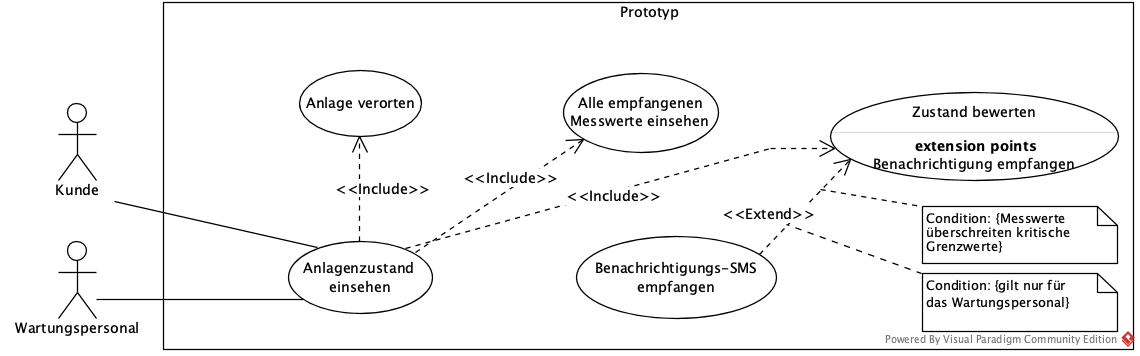
\includegraphics[width=\paperwidth]{use_case_basic.png}}
  \caption[Use Case Diagramm der Kontextebene]{Use Case Diagramm der Kontextebene}
  \label{usecase_basic}
\end{figure}
\noindent Gelöst werden die Probleme jedoch in erster Linie durch die Verfügbarkeit einer intelligenten Verwaltungsschale über der physischen Anlage nach dem Konzept der Industrie-4.0-Komponente (s. Abschnitt \ref{rami}).
Ein wesentliches Merkmal von Industrie-4.0-Projekten ist die Interdisziplinarität und Komplexität (K-P-3). Für den Aufbau einer Strategie und die Bewältigung der Herausforderungen, die ein komplexes System stellt, wird eine von Politik und Wirtschaft entwickelte Referenzarchitektur als Hilfe herangezogen. Das \ac{rami} bildet (s. Abschnitt \ref{rami}) eine wichtige Entscheidungsgrundlage für die Beurteilung der Eignung (K-P-4) der prototypischen Architektur eines solchen Systems. Da die Umsetzungsstrategie der Plattform Industrie 4.0 \citep{BITKOM2015} jedoch erneuerbare Energien nicht berücksichtigt, aber die Abhängigkeit von fluktuierenden Regularien (K-P-2) besteht, soll eine unternehmensspezifische Digitalisierungslösug entwickelt werden. Weiterhin ist die grobe Struktur des Zielsystems maßgeblich durch die Vorgabe von SAP Leonardo als digitale Schicht für physische Anlagen bestimmt. Da der \ac{sa} erst innerhalb der Systemgrenzen mit dem System interagiert, werden dessen Anwendungsfälle in der Systemebene konkretisiert.

\begin{table}[H]
  \begin{tabularx}{\textwidth}{@{}lXp{2cm}@{}}
      \toprule
      ID                & Lösung & Quelle \\
      \midrule
      \textbf{K-L-1}              &   Intelligente Verwaltungsschale für die reale Anlage & \textit{K-P-1}                \\
      \multicolumn{1}{r}{K-L-1.1} &  Der Zustand und zugehörige Daten sollen jederzeit einsehbar sein & \textit{K-P-1.1}\\
      \multicolumn{1}{r}{K-L-1.2} & Der Zustand der Anlage soll bewertbar sein & \textit{K-P-1.2}\\
      \multicolumn{1}{r}{K-L-1.3} & Zustandsveränderungen sollen unverzüglich gemeldet werden & \textit{K-P-1.3}\\
      \textbf{K-L-2}              & Aufbau eines unternehmensspezifischen Digitalisierungslösung    & \textit{K-P-2}                \\
      \textbf{K-L-3}              & IT-Sicht des RAMI 4.0 und Industrie-4.0-Komponente           & \textit{K-P-3}                \\
      \textbf{K-L-4}              &  Prototypische Architekturvorlage für IoT-Projekte & \textit{K-P-4} \\
      \multicolumn{1}{r}{K-L-4.1} &  Messinstrument zur Simulation einer realen Anlage & \textit{K-P-4.2}\\
      \addlinespace
      \bottomrule
  \end{tabularx}
  \label{kontext_losung}
  \caption{Lösungen aus Kontextebene}
\end{table}

\paragraph{Anforderungen}

Die Anforderungsdefinition in der Kontextebene ist von hoher Abstraktion geprägt. Sie entstehen aus den wesentlichen Problemen, die das Zielsystem zu lösen hat. Es wird zunächst ein grober Überblick über die wichtigsten Anforderungen an das Gesamtsystem gegeben, um eine Orientierung für die Anforderungserhebung auf Systemebene zu schaffen. Nach \citet{Doleski2016} gibt es drei wesentliche Anforderungen an Energieunternehmen. Zum einen gilt es die Informationsflut aus der dezentralen Produktion zu bewältigen. Bezogen auf das Zielsystem bedeutet dies, Messwerte aus der Anlage in einem digitalen Zwilling visuell bereitzustellen. Außerdem müssen diese Informationen Wissen erzeugen. Das System muss dies durch die Bereitstellung von prädiktiven Informationen und durch Reaktion auf kritische Zustände ermöglichen. Zudem müssen aus den Informationen relevante Erkenntnisse für die Unternehmensführung gewonnen werden. Dafür muss das Zielsystem eine Möglichkeit für die Einbindung von intelligenten Diensten zur Datenverarbeitung aufweisen. Für einen besseren Überblick sind die Anforderungen in Tabelle \ref{kontext_anforderungen} gelistet.

\begin{table}[ht!]
  \begin{tabularx}{\textwidth}{@{}lXp{2cm}@{}}
      \toprule
      ID                & Anforderung & Quelle \\
      \midrule
      % Funktionale Anforderungen
      \textbf{K-FA-1}              &   Das System muss dem Nutzer Zugriff auf den digitalen Zwilling der Anlage gewähren.  & \textit{K-P-1}                \\
      \multicolumn{1}{r}{K-FA-1.1} &  Das Sytem muss dem Nutzer die aktuellen Messewerte in Echtzeit anzeigen.    & \textit{K-P-1.1}\\
      \multicolumn{1}{r}{K-FA-1.2} & Das System muss dem Nutzer die Verortung der Anlage ermöglichen. \\
      \multicolumn{1}{r}{K-FA-1.3} & Das System muss dem Nutzer prädiktive Informationen liefern.\\
      \multicolumn{1}{r}{K-FA-1.4} & Das System muss dem Nutzer die Reaktion auf kritische Zustände in Echtzeit ermöglichen.  & \textit{K-P-1.2}\\
      % Qualitative Anforderungen
      \textbf{K-QA-1}              & Die Architektur des Systems muss dem \ac{sa} die flexible Anpassung an Änderungen erlauben.     & \textit{K-P-2}                \\
      \textbf{K-QA-2}              & Die Architektur des Systems muss dem \ac{sa} die Einbindung neuer Anlagen erlauben.           & \textit{Auftraggeber}                \\
      \textbf{K-QA-3}              &  Die Architektur des System muss dem \ac{sa} die Einbindung von intelligenten Diensten erlauben.  & \textit{K-P-4.1} \\
      \textbf{K-QA-4}              &  Die Architektur des System muss dem \ac{sa} erlauben, das System um Funktionen zu erweitern.  & \textit{K-P-4.1} \\
      % Rahmenbedingungen
      \textbf{K-RA-1}              & Für die Umsetzung des Prototypen muss die SAP Leonardo IoT Foundation verwendet werden.       & \textit{K-P-4} \\
      \textbf{K-RA-2}              & Die Architektur des Systems muss mit \ac{rami} konform sein.      & \textit{K-P-3} \\
      \textbf{K-RA-3}              & Die Simulation muss die Eigenschaften einer Industrie-4.0-Komponente aufweisen.      & \textit{K-P-4.2} \\
      \addlinespace
      \bottomrule
  \end{tabularx}
  \caption{Anforderungen aus Kontextebene}
  \label{kontext_anforderungen}
\end{table}

\newpage

\subsubsection{Systemebene}
Um den inneren logischen Aufbau des Systems zu spezifizieren, müssen die Lösungen und Anforderungen der Kontextebene erneut in zu lösende Probleme zerlegt werden. Anschließend wird das Systemmodell vorgestellt, welches mit seinen Schnittstellen, Funktionen und Datenstrukturen die Probleme lösen soll. Da aus der Spezifikation der Systemfunktionen sich neue Anwendungsfälle ergeben, werden diese ebenfalls spezifiziert. Schließlich werden die Anforderungen an das System definiert.

\paragraph{Problemstellungen} Damit das System die Anforderungen der des Systemkontextes lösen kann, muss es spezielle Probleme lösen. Das Hauptproblem ist die Virtualisierung eines physischen Assets mitsamt der zugehörigen Messdaten. Unabhängig davon, wo sich der Nutzer befindet, soll er jederzeit den Zustand der Anlage durch den digitalen Zwilling einsehen können. Dabei soll es dem Nutzer ermöglicht werden, den digitalen Zwilling eindeutig einer realen Anlage zuzuordnen. Um einen Mehrwert aus den gemessenen Daten zu erlangen, muss das System die Bedeutung bestimmter Daten erkennen und ggf. eine Benachrichtigung versenden.

\begin{table}[ht!]
  \begin{tabularx}{\textwidth}{@{}lXp{2cm}@{}}
      \toprule
      ID                & Problem & Quelle \\
      \midrule
      \textbf{S-P-1}              &       Übergabe des pyhsischen Assets in die digitale Welt               &  K-FA-1               \\
      \multicolumn{1}{r}{S-P1.1} &  Erzeugung eines cyber-physischen Systems als Messinstrument  & \\
      \multicolumn{1}{r}{S-P1.1} &  Empfang aller Zustandsdaten der Anlage     \\
      \multicolumn{1}{r}{S-P1.2} &  Identifikation der Anlage     \\
      \multicolumn{1}{r}{S-P1.3} &  Erkennung der Bedeutung eines Messwerts  & K-FA.13\\
      \multicolumn{1}{r}{S-P1.4} &  Orts- und zeitunabhängige Anzeige der Zustandsdaten einer Anlage     \\
      \multicolumn{1}{r}{S-P1.5} &  Verortung einer Anlage & K-FA.1.2\\
      \multicolumn{1}{r}{S-P1.6} &  Erkennung der Grenzüberschreitung eines Messwerts & K-FA-1.4\\
      \multicolumn{1}{r}{S-P1.7} &  Erkennung der Notwendigkeit einer erneuten Benachrichtigung\\
      \textbf{S-P-2}              &  Bereitstellung einer flexiblen Systemarchitektur  & K-QA \\
      \textbf{S-P-3}              &  Bereitstellung einer standard-konformen Systemarchitektur K-RA \\
      \addlinespace
      \bottomrule
  \end{tabularx}
  \label{system_probleme}
  \caption{Probleme aus Systemebene}

\end{table}


\paragraph{Systemmodell}

Damit das System die Anwendungsfälle aus Abbildung \ref{usecase_basic} ermöglichen kann, enthält es im Inneren bestimmte Funktionen, Schnittstellen und Datenstrukturen. Von der Virtualisierung der Anlage bis zur Präsentation für den Nutzer fließen viele Daten. Der Fluss der Daten über die Funktionen und Schnittstellen ergibt ein erstes grobes Systemmodell (s.Abbildung \ref{dataflow}). Die gelben Objekte repräsentieren sind Schnittstellen, die die Verbindung des Systems mit der Umwelt beschreiben. Über die Funktionen (grün) fließen die Daten an die Datenspeicher (rot), bis sie schließlich bei den Nutzern ankommen. Dieses Diagramm dient nicht dazu, den Datenfluss zu kontrollieren, d.h. Bedingungen zu setzen. Es soll lediglich einen Überblick über den Aufbau des Systems geben.

\begin{figure}[ht!]
  \centering
  \noindent\makebox[\textwidth]{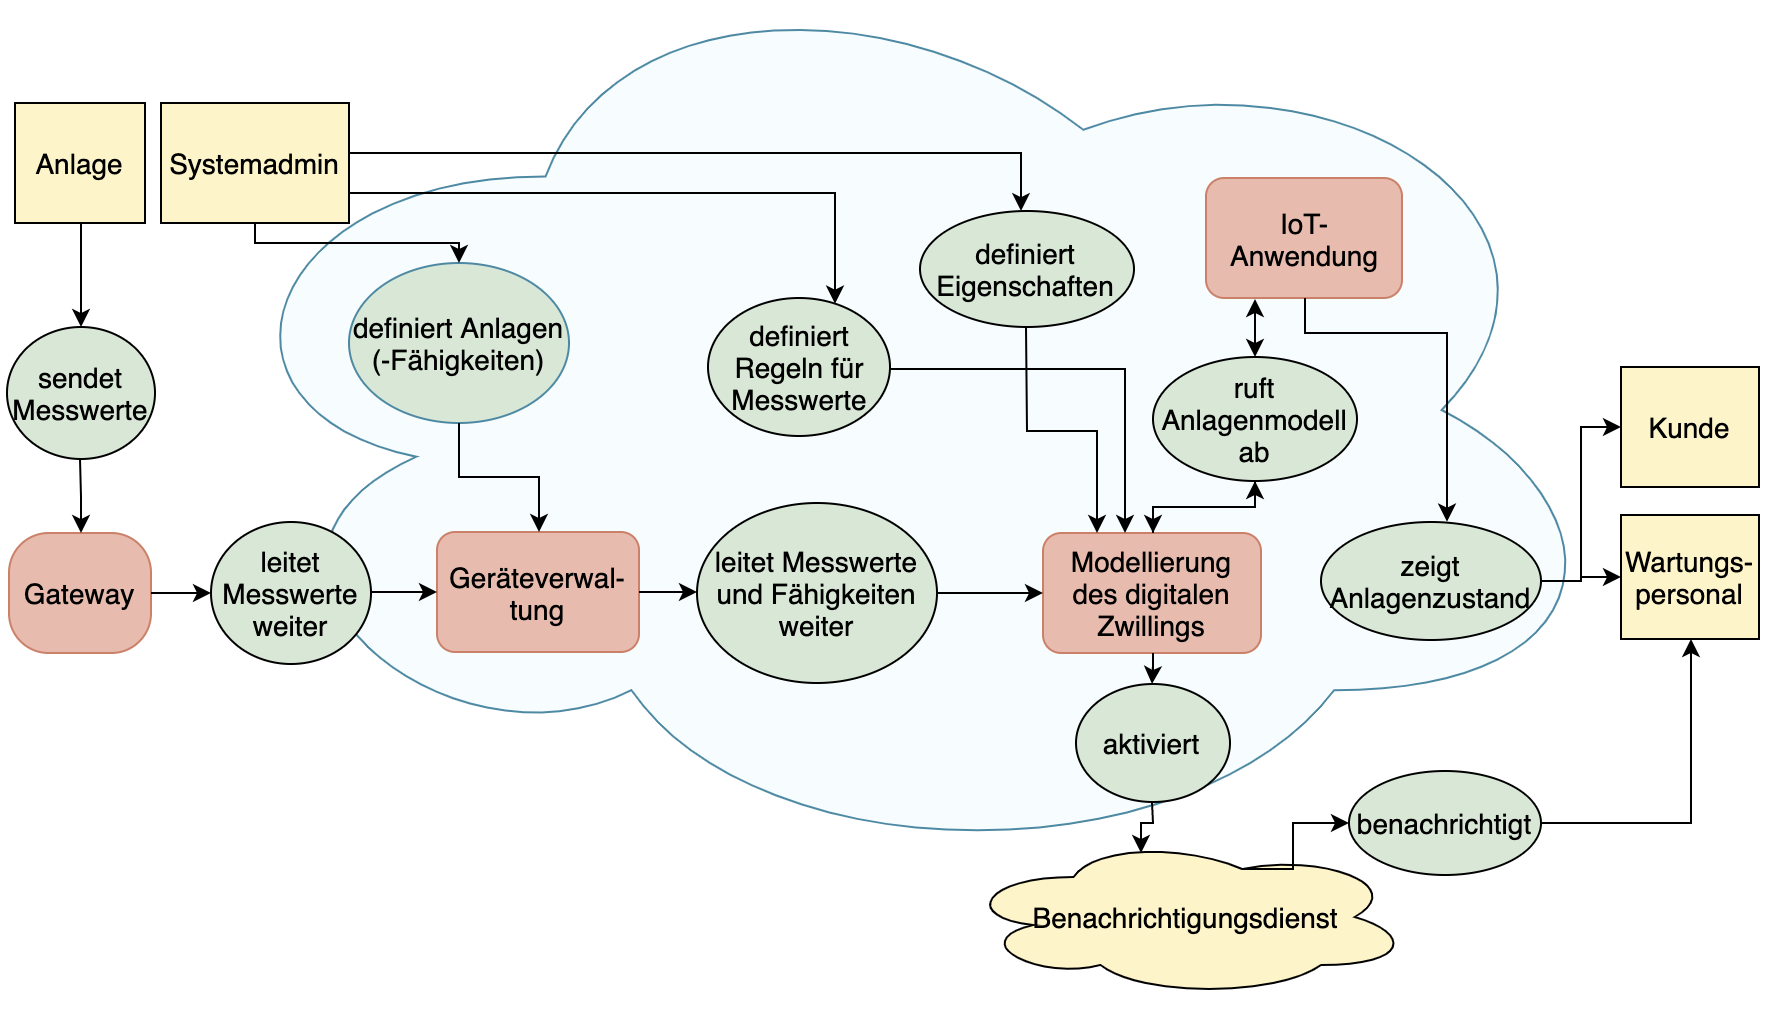
\includegraphics[width=\paperwidth]{data_flow.png}}
  \caption[Datenflussdiagramm]{Datenflussdiagramm}
  \label{dataflow}
\end{figure}

\noindent Aus dem Diagramm sind die \textbf{Schnittstellen} Anlage, Systemadmin, die Nutzer und der Benachrichtigungsdienst zu entnehmen. Technisch gesehen existieren noch andere Schnittstellen, die Daten austauschen.

\begin{enumerate}
  \item Sensoren zu \textit{Anlage}: Messwerte werden durch Computerverarbeitung Eigenschaften der Anlage zugeordnet. \begin{itemize}
    \item 1 Anlage besteht aus n Sensoren und 1 Gateway
  \end{itemize}
  \item Anlage zur Cloud: Messwerte \textit{Gateway} werden über ein Protokoll an eine Destination in der Cloud gesendet
  \item Cloud zur Geräteverwaltung
  \item Cloud zum digitalen Zwilling: \textit{Message Processing}
  \item Regeln zum digitalen Zwilling
  \item Events zum digitalen Zwilling
  \item Benachrichtigungsdienst zu dem digitalen Zwilling/Messwerten
  \item Nutzer zur IoT-App
\end{enumerate}

Funktionen: Datenflussdiagramm
\begin{itemize}
  \item Funktionen im Sinne der Verarbeitung von Daten
  \item werden direkt durch Schnittstellen oder andere Funktionen ausgelöst
  \item Verbunden mit Anwendungsfällen aus Kontextebene
  \item Andere Funktionen aus Systemebene
  \item Anwendungfälle auf Systemebene
\end{itemize}

Datenstrukturen

\begin{itemize}
  \item sämtliche im System gespeicherte Daten: Datum und Bezeichner
  \item ER-Modelle: Device Modell mit Angepassten Capabilties
\end{itemize}



Abbildung s. \ref{ebenen_i40}

\begin{figure}[h]
  \centering
  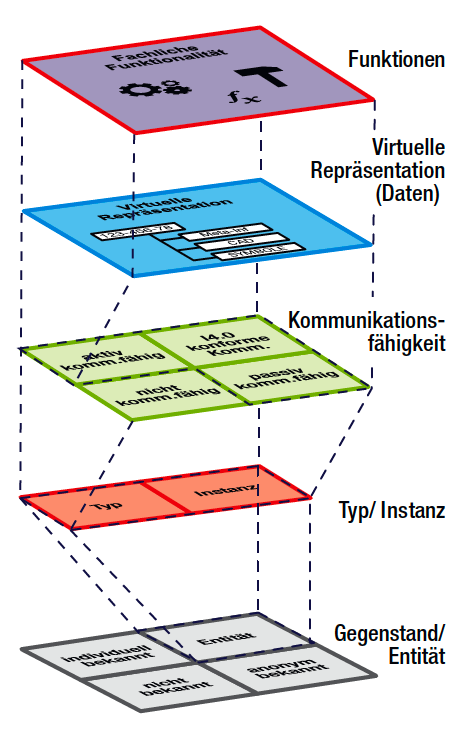
\includegraphics[width=0.5\linewidth]{Ebenen_I40_Kompo.png}
  \caption[Ebenen der Industrie-4.0-Komponente]{Ebenen der Industrie-4.0-Komponente \citep[S. 52]{BITKOM2015}}
  \label{ebenen_i40}
\end{figure}

\paragraph{Aufbau der Nutzeroberfläche}
\paragraph{Anwendungsfälle}

\begin{figure}[ht!]
  \centering
  \noindent\makebox[\textwidth]{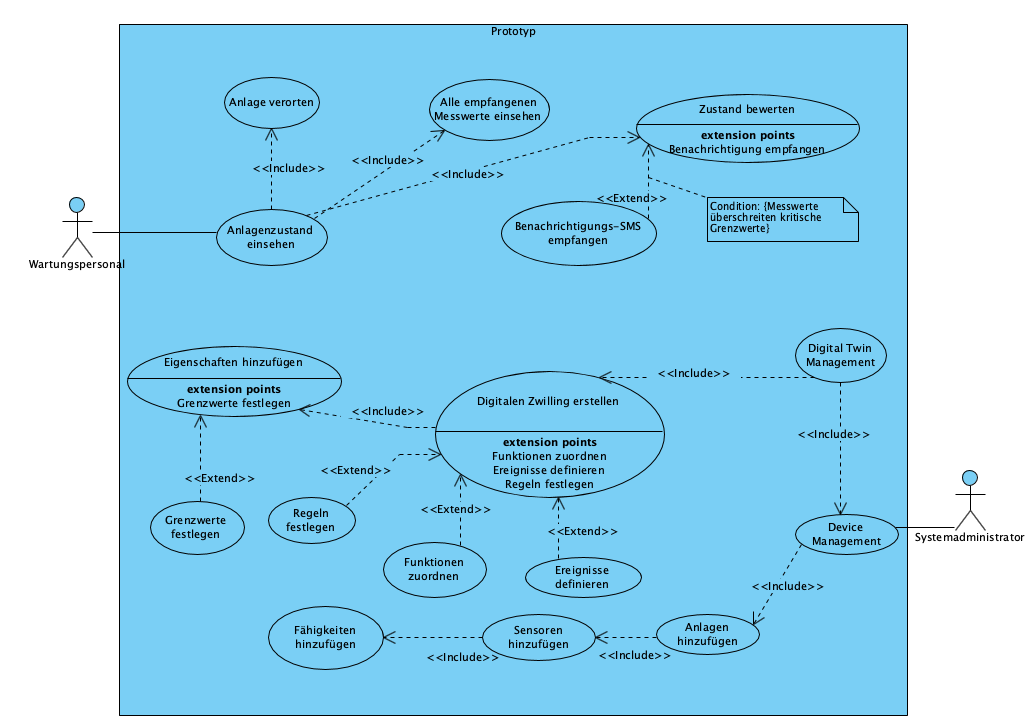
\includegraphics[width=\paperwidth]{usecase_ext1.png}}
  \caption[Erweitertes Use Case Diagramm auf Systemebene]{Erweitertes Use Case Diagramm auf Systemebene}
  \label{usecasediagram}
\end{figure}
\paragraph{Anforderungen}

In Bezug auf Datenstrukturen, Schnittstellen, Funktionen, Elemente in Nutzeroberfläche

\begin{table}[ht!]
  \begin{tabularx}{\textwidth}{@{}lXp{2cm}@{}}
      \toprule
      ID                & Anforderung & Quelle \\
      \midrule
      % Funktionale Anforderungen
      \textbf{S-FA-1}              &  Das System muss dem Nutzer Zugriff auf den digitalen Zwilling der Anlage gewähren.  & \textit{K-P-1}                \\
      \multicolumn{1}{r}{S-FA-1.1} &  Das Sytem muss dem Nutzer die aktuellen Messewerte in Echtzeit anzeigen.    & \textit{K-P-1.1}\\
      \multicolumn{1}{r}{S-FA-1.2} & Das System muss dem Nutzer die Verortung der Anlage ermöglichen. \\
      \multicolumn{1}{r}{S-FA-1.3} & Das System muss dem Nutzer prädiktive Informationen liefern.\\
      \multicolumn{1}{r}{S-FA-1.4} & Das System muss dem Nutzer die Reaktion auf kritische Zustände in Echtzeit ermöglichen.  & \textit{K-P-1.2}\\
      % Qualitative Anforderungen
      \textbf{S-QA-1}              & Die Architektur des Systems muss dem \ac{sa} die flexible Anpassung an Änderungen erlauben.     & \textit{K-P-2}                \\
      \textbf{S-QA-2}              & Die Architektur des Systems muss dem \ac{sa} die Einbindung neuer Anlagen erlauben.           & \textit{Auftraggeber}                \\
      \textbf{S-QA-3}              &  Die Architektur des System muss dem \ac{sa} die Einbindung von intelligenten Diensten erlauben.  & \textit{K-P-4.1} \\
      \textbf{S-QA-4}              &  Die Architektur des System muss dem \ac{sa} erlauben, das System um Funktionen zu erweitern.  & \textit{K-P-4.1} \\
      % Rahmenbedingungen
      \textbf{S-RA-1}              & Für die Umsetzung des Prototypen muss die SAP Leonardo IoT Foundation verwendet werden.       & \textit{K-P-4} \\
      \textbf{S-RA-2}              & Die Architektur des Systems muss mit \ac{rami} konform sein.      & \textit{K-P-3} \\
      \textbf{S-RA-3}              & Die Simulation muss die Eigenschaften einer Industrie-4.0-Komponente aufweisen.      & \textit{K-P-4.2} \\
      \addlinespace
      \bottomrule
  \end{tabularx}
  \caption{Anforderungen aus Kontextebene}
  \label{kontext_anforderungen}
\end{table}

\begin{itemize}
  \item logischer Aufbau des Systems
  \item Problemstellung/Ziele: ergeben sich aus Anforderungen der Kontextebene
  \item Systemmodell: Schnittstellen, Funktionen, Datenstrukturen
  \item Schnittstellen: Verbindung des Systems zur Umwelt (technisch und Nutzer) -> wurden im Kontextmodell definiert
  \item technisch: Beschreibung der Daten, die mit Umwelt ausgetauscht werden
  \item Nutzer: bennen
  \item Funktionen: Funktionalitäten des Systems, Datenverarbeitung
  \item Funktionen verbunden mit Anwendungsfällen auf Kontextebene
  \item oder andere Funktionen der Systemebene: zentralisierte Funktiona
  \item oder Anwendungsfälle auf Systemebene: Funktion realisiert Teilfunktionalität auf Systemebene
  \item triviale Funktionnen wie Logout oder Login nur kurz -> Fokus auf geschäftskritische Funktionen
  \item Funktion kann nur diejenigen Daten verarbeiten, welche in Datenstrukturen und Schnittstellen zur Verfügung gestellt werden
  \item Datenstrukturen: ER-Diagramm oder Klassenmodelle
  \item Aufbau Nutzeroberflächen: falls vorhanden, setzt Schnittstellen und Daten voraus
  \item Anwendungsfälle auf Kontextebene können auf Systemebene konkretisiert werden
  \item Anforderungen: Anforderungen an innere Bestandteile des Systems
\end{itemize}
Anpassbar, Änderbar, Benutzbar, Genau, Performanz, Sicherheit, Übertragbarkeit, Zuverlässigkeit

Datenflussdiagramm

% Technische Ebene
\subsubsection{Technische Ebene}
Das ist eher Teil der Software-Architektur, daher nur ganz kurz fassen

\paragraph{Problemstellungen und Ziele}
Ergeben sich aus Anforderungen der Systemebene

\begin{table}[ht!]
  \begin{tabularx}{\textwidth}{@{}lXp{2cm}@{}}
      \toprule
      ID                & Problem & Quelle \\
      \midrule
      \textbf{S-P-1}              &       Übergabe des pyhsischen Asssets in die digitale Welt               & \textit{Branche}                \\
      \multicolumn{1}{r}{T-P1.1} &  Erzeugung eines cyber-physischen Systems als Messinstrument \\
      \multicolumn{1}{r}{T-P1.1} &  Empfang der Zustandsdaten der Anlage     \\
      \multicolumn{1}{r}{T-P1.2} &  Erkennung der Bedeutung eines Messwerts \\
      \multicolumn{1}{r}{T-P1.3} &  Ortsunabhängige Anzeige der Zustandsdaten einer Anlage     \\
      \multicolumn{1}{r}{T-P1.4} &  Verortung einer Anlage \\
      \multicolumn{1}{r}{T-P1.5} &  Erkennung der Grenzüberschreitung eines Messwerts \\
      \multicolumn{1}{r}{T-P1.6} &  Erkennung der Notwendigkeit einer erneuten Benachrichtigung\\
      \textbf{S-T-2}              &  Bereitstellung einer flexiblen Systemarchitektur   \\
      \textbf{S-T-3}              &  Bereitstellung einer standard-konformen Systemarchitektur \\
      \addlinespace
      \bottomrule
  \end{tabularx}
  \label{system_probleme}
  \caption{Probleme aus technischer Ebene}
\end{table}
\paragraph{Technischer Aufbau des Systems}
verwendete Technologien und konkrete Ausprägung des Systems
z.B. technische Architekturbeschreibungen, technische Datenmodelle oder verwendete Hardwaresysteme

\paragraph{Anforderungen}
müssen sich stets an die Elemente des technischen Aufbaus beziehen
\begin{itemize}
  \item technische Ebene z.B. Datenbanken bestimmter Hersteller oder Vorgaben zur Umsetzungstechnolgie wie Programmiersprachen oder Frameworks -> in diesem Fall SAP Leonardo und SCP
  \item Problemstellung/Ziele
  \item Technischer aufbau des Systems: technische Architekturbeschreibungen, technische Datenmodelle, verwendete Hardwaresysteme
  \item Elemente des Sytemmodells vollständig abdecken
\end{itemize}



Was muss das System können? An RAMI orientieren -> Was muss erfüllt werden ?
Scada macht über Protokolle und Schnittstellen Telemetriedaten der Windenergieanlage
schreibt das Lokal in eine DB und erzeugt Alarmmeldungen
quittieren lokal am Rechner
alle 10 Minuten --> mit Leonardo schnellere Reaktion in Echtzeit
50 Hz Frequenz -> muss gehalten werden, um schnell auf Probleme reagieren zu können


\begin{itemize}
  \item erneuerbare Energien werden von der Plattform Industrie 4.0 kaum berücksichtigt !
  \item Was Kann SCADA-System? daten erfassen, an cloud senden, verarbeiten, digitaler zwilling unf steuern, aktionen und regeln für predictive Maintenance
  \item Fähigkeit, große Datenmengen auch offline zu verarbeiten -> Latenzprobleme
  \item ANFORDERUNG! WENN DIE Anlagen ins Smart Grid aufgenommen werden sollen, müssen sie Kommunikationsfähig sein!!!!
  \item Aus Requirements Engineering S. 10: Simulation vor Inbetriebnahme, um Fehler in Anforderungsanalyse festzustellen, damit Change Requests gemacht werden können
  \item Bei Anlagen, die mehrere Millionen Euro kosten, sind anders als in Software Mechanik und Elektronik eingebaut. Ein Change Request wäre viel zu teuer
  \item Anforderungsanalyse der Simulation beseitigt die Risiken nicht vollständig, da die Simulation nur so gut ist, wie man sich vorher Gedanken gemacht hat
  \item Welche Anforderungen ergeben sich aus dem Wandel?
  \item Anforderungen wie predictive Maintenance und Bezug auf RAMI 4.0.
  \item SAP als Tool, da Energiesektor hauptsächlich \acf{sapisu}
  \item Industrie 4.0-Komponente (Bitkom s. 52) mit verschiedenen Ebenene
\end{itemize}

\textbf{Anforderungen an Versorgungsunternehmen im Energiesystem der Zukunft \citep[S. 19]{Doleski2016}}

\paragraph{Merkmale von Akteuren in der digitalen Welt}
\begin{itemize}
  \item Allgegenwärtige Informationsverfügbarkeit
  \item Soziale Visualisierung1
  \item Absolute Mobilität
  \item Permanente Erreichbarkeit
  \item Lokalisierung
  \item Leistungsfähige Technologien
\end{itemize}

\paragraph{Wesentliche Herausforderungen für Energieunternehmen \citep[S. 21]{Doleski2016}}
\begin{enumerate}
  \item \textbf{Informationsflut}: zunehmendes Informationsangebot kann nicht oder nur bedingt aufgenommen werden
  \item \textbf{Informationsverarbeitung}: zunehmendes Informationsangebot kann nicht zu Wissen verarbeitet werden
  \item \textbf{Informationssysteme}: bestehende Informationssysteme liefern oftmals keine relevanten Informationen für die Unternehmensführung
\end{enumerate}
